
\chapter{Architektura a technologie} \label{archtech}

\section{Architektura řešení} \label{architektura_reseni}

\begin{figure} \centering
  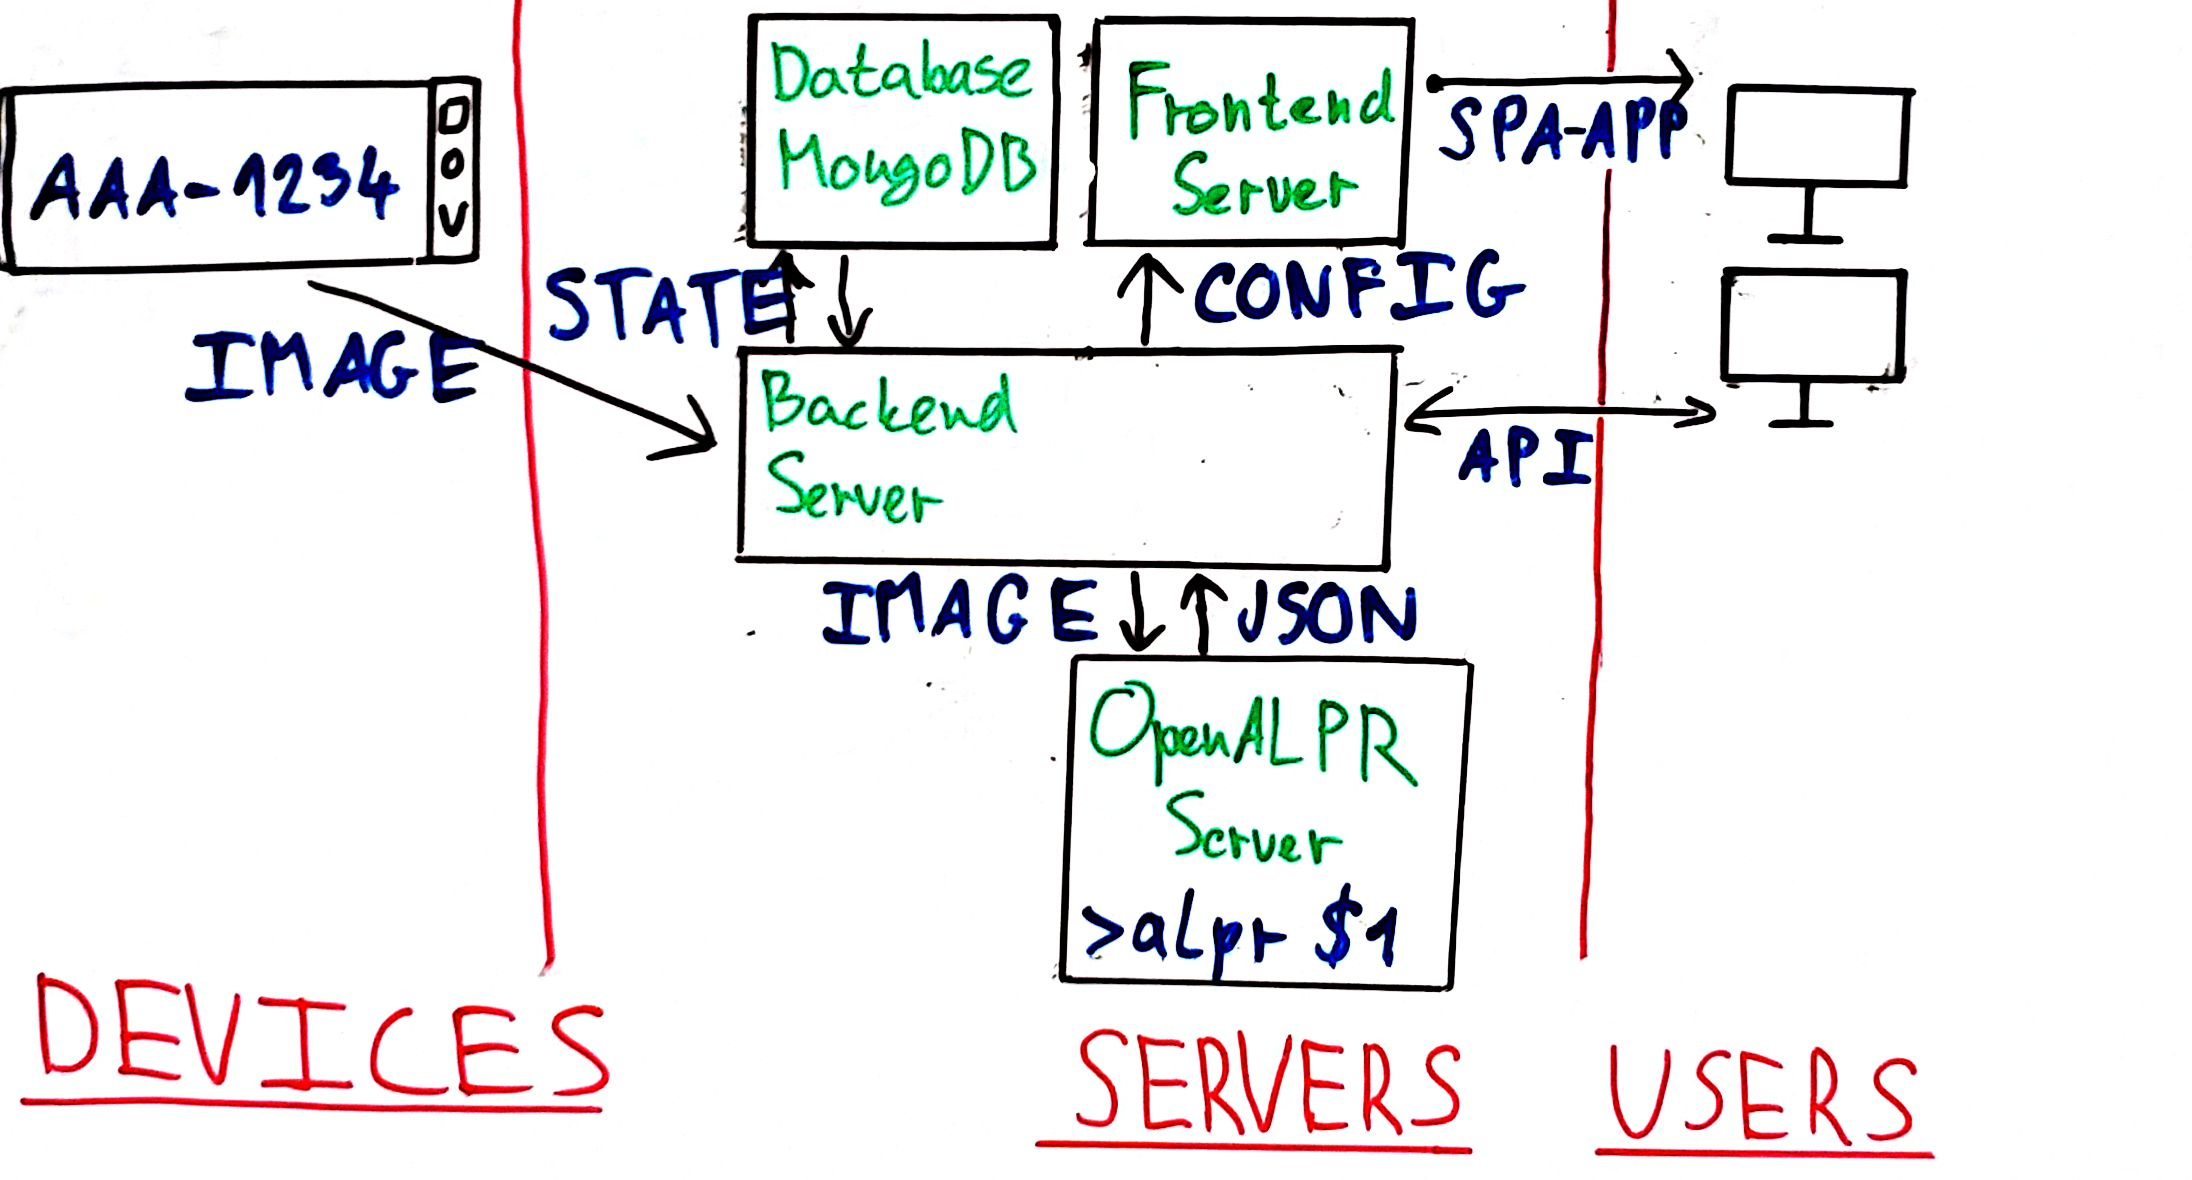
\includegraphics[width=145mm]{../img/architecture_drawing.jpg}
  \caption{Diagram komponent a jejich komunikace.}
  \label{fig:architecture_drawing}
\end{figure}

\noindent
Parkovací systém se skládá z následujících částí, které si nyní popíšeme stručně a detailněji v
následujících kapitolách.
Jednotlivé komponenty spolu komunikují pomocí HTTP.
Obrázek \ref{fig:architecture_drawing} ukazuje tyto části a nastiňuje obsah komunikace.

\begin{itemize}
  \setlength\itemsep{.05em}
  \item \textbf{Backend} je středobodem celého systému -- komunikuje se všemi ostatními komponentami.
  Zajišťuje business logiku aplikace, autentizaci i autorizaci uživatelů i zařízení
  a persistenci dat do databáze.
  \begin{itemize}
    \setlength\itemsep{.05em}
    \item \textbf{Databáze} slouží k ukládání a čtení dat.
    \item \textbf{OpenALPR Server} obstarává přístup
          ke knihovně OpenALPR přes HTTP, která rozpoznává SPZ.
  \end{itemize}
  \item \textbf{Mobilní aplikace} je určená pro platformu Android a posílá obrazová data na backend,
        kde jsou zpracována.
  \item \textbf{Frontend} je rozhraní mezi celým systémem a správcem parkoviště.
\end{itemize}

\section{Technologie}

\subsection{Databáze}

\noindent
Databáze MongoDB byla vybrána, protože data se budou převážně zapisovat a bude potřeba v nich rychle
hledat a provádět agregační dotazy.
MongoDB je takzvaná NoSQL databáze -- k dotazování se nepoužívá SQL, nýbrž vlastní způsob dotazování v
JSON. Základní datovou jednotkou je JSON/BSON dokument.
Mimo jiné umožňuje provoz několika spolupracujících instancí, zálohování apod. \citep[][]{MongoDB}

\subsection{Backend} \label{backend}

\noindent
Jako programovací jazyk pro backend byl zvolen staticky typovaný Typescript kvůli rychlosti vývoje
a množství knihoven, které poskytuje ekosystém Node.js. \citep[][]{Typescript} \citep[][]{Nodejs}

Pro definici databázových modelů a komunikaci s databází byla kvůli své vyspělosti a skvělé funkcionalitě zvolena
knihovna mongoose. \citep[][]{Mongoose}

Primárním způsobem komunikace s frontendem
je dotazovací jazyk GraphQL, který přináší ucelený popis poskytovaných dat pomocí kontroly typů a
expresivních dotazů, jejichž odpověď má stejný ``tvar'' v JSON formátu. 
Obrázek \ref{fig:graphql_example} ukazuje dotaz hledání uživatele podle jména.

\begin{figure} \centering
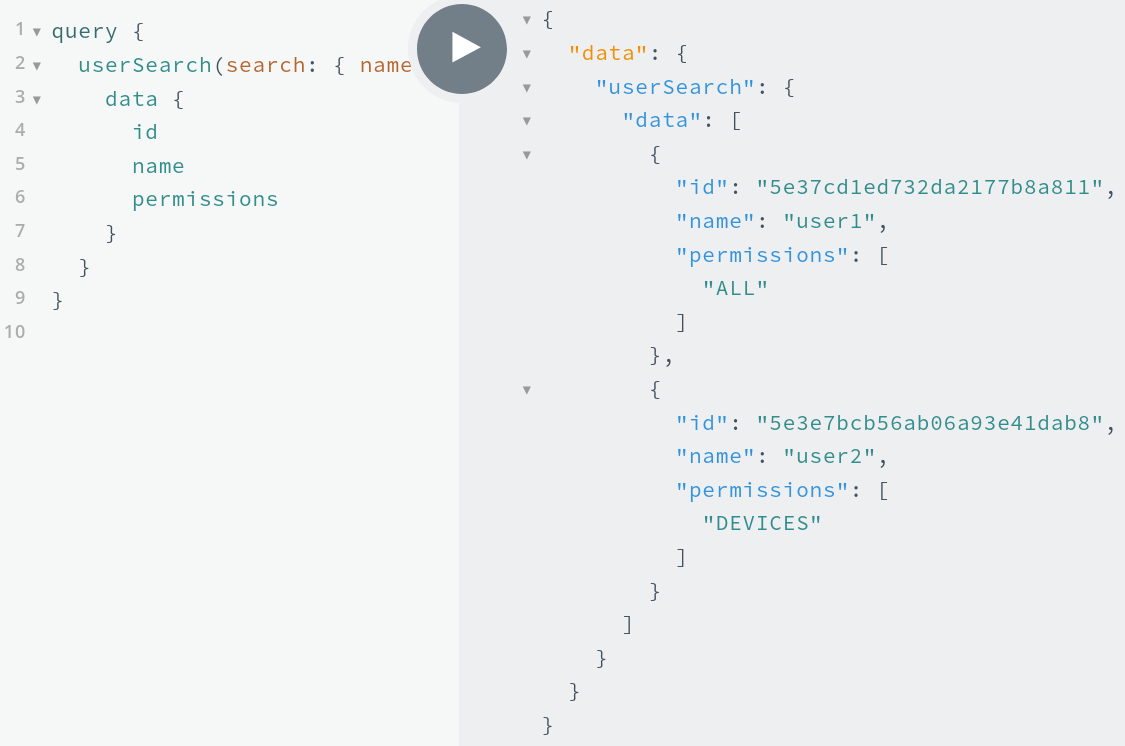
\includegraphics[width=145mm]{../img/graphql_example.png}
\caption{Příklad GraphQL dotazu (vlevo) a odpovědi (vpravo). Screenshot z nástroje GraphQL Playground.}
\label{fig:graphql_example}
\end{figure}

Model uživatele může mít i další atributy, ale GraphQL vrátí přesně ty údaje, na které se klient zeptal.
Tento triviální příklad neukazuje další funkce jako mutace dat, dědičnost typů, více dotazů v jedné HTTP žádosti
a mnoho dalších funkcí.
GraphQL je pouze specifikace vytvořená společností Facebook a má několik
implementací. \citep[][]{GraphQLDoc} Pro tento projekt byla zvolena implementace Apollo,
protože poskytuje knihovnu pro backend i frontend. \citep[][]{Apollo}

Jelikož GraphQL posílá odpovědi v JSON, není vhodné pro posílání obrázků. Je to možné za využití base64 kódování,
ale přes síť se přenese více bytů, než při použití obvyklého způsobu přes HTTP. Z toho důvodu pro posílání
obrázků bude mít backend i jiné endpointy.

\subsection{Frontend} \label{frontend}

\noindent
Pro frontend byl jako u backendu vybrán Typescript ze stejných důvodů. Webové rozhraní
je takzvaná SPA (z angl. Single-Page-Application), což znamená, že uživateli se obsah mění dynamicky
bez načítání dalších stránek.

Renderování zajišťuje knihovna React, která od klasického přístupu, kdy se odděluje HTML a Javascript do separátních
souborů, mandatuje, že v jednom souboru je jedna komponenta se vším svým HTML a logikou ve formě Javascriptu nebo
Typescriptu. \citep[][]{Reactjs}
Pomocí další knihovny typestyle pak můžeme do stejného souboru psát i typované CSS.\citep[][]{typestyle}

Aby bylo možné snadno sdílet mezi komponentami stav, byla pro takzvaný \textit{state-management} zvolena knihovna Redux.
\citep[][]{ReduxCore}
Diagram na obrázku \ref{fig:react_redux_dataflow} ukazuje tok dat mezi Reactem a Reduxem.
Tato architektura zároveň umožňuje testovatelnost -- můžeme jednoduše ověřit, zdali byla akce
například po kliknutí na tlačítko komponenty vyvolána, a jak komponenta reagovala na změnu stavu.

Jelikož je aplikace vyvíjena pro správce systému a ne pro velké množství uživatelů, můžeme si dovolit
klást menší nároky na velikost aplikace (tj. můžeme přidávat i velké knihovny), což velice usnadní vývoj.

\begin{figure}[!htb] \centering
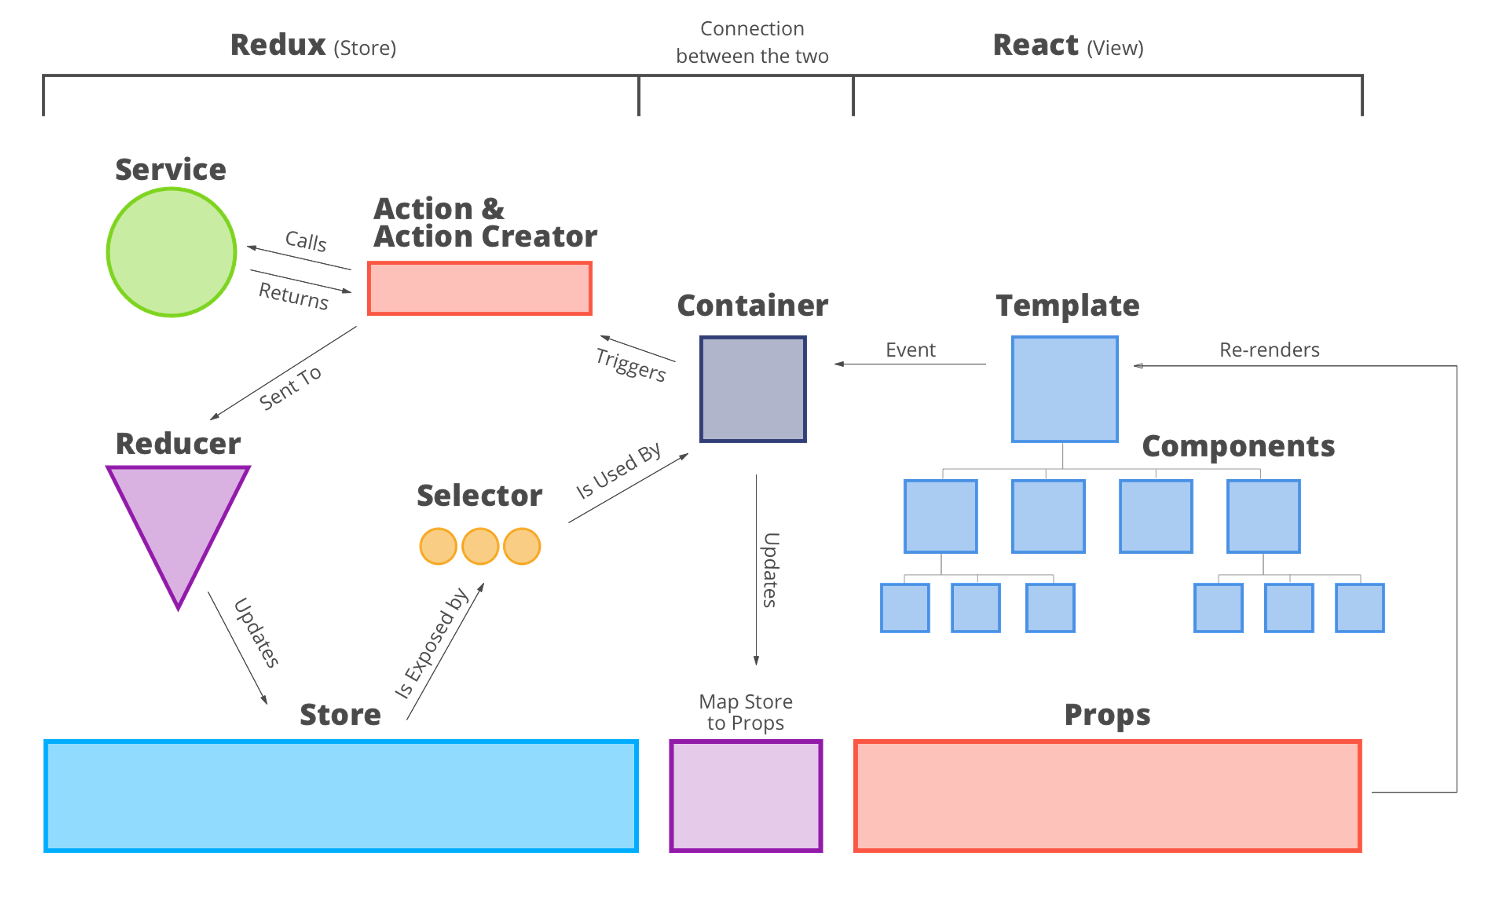
\includegraphics[width=145mm]{../img/react-redux-architecture.png}
\caption[Spojení React a Redux.]{Spojení React a Redux. \citep[][]{react_redux_dataflow}
Komponenty vyvolávají akce pomocí \textit{action-creators}, akce jsou předány prostým funkcím zvaným \textit{reducers},
ty aktualizují stav. Každá komponenta napojená
na Redux má \textit{selector} funkci, pokud se výstup z \textit{selector} funkce aktualizuje, komponenta je přerenderována Reactem.
V obrázku je prvek zvaný \textbf{Container}, ten je HOF (abbrv. Higher-Order-Function) pro komponentu a dodává jí přístup ke stavu a vytváření akcí.
Reakce na akci může být i dotaz na server nebo jiný vedlejší efekt mimo komponentu.}
\label{fig:react_redux_dataflow}
\end{figure}

\subsection{Mobilní aplikce} \label{mobile_app}

\noindent
Mobilní aplikace, která je určena pro platformu Android, měla volbu jazyka omezenou na Javu, Kotlin a C++.
Rychlost C++ není potřeba a navíc autor s tímto nízkoúrovňovým jazykem nemá takové zkušenosti.
Kotlin oproti Javě umožňuje přímočarejší přístup k prvkům uživatelského rozhraní, a proto byl zvolen.

Jediným úkolem mobilní aplikace je v pravidelném intervalu pořizovat snímky fotoaparátem a posílat je na
backend, který je patřičně zpracuje.

\subsection{Detekce SPZ}

\noindent
Detekci SPZ bude zajišťovat knihovna OpenALPR, jejímž vstupem je obrázek a popřípadě
parametry jako úhel kamery apod.
\citep[][]{OpenALPR}

Ke zbytku aplikace bude připojena malým HTTP serverem, jenž byl převzat a upraven.
Ten umožňuje poslat pomocí HTTP obrázek a obdržet JSON s SPZ daty a souřadnicemi detekované SPZ.
Samotný server ke knihovně přistupuje zavoláním binárky \textit{alpr}, který jako argument přijme cestu k
obrázku, ve kterém hledáme SPZ. \citep[][]{OpenALPR_Server}

Alternativní a lepší způsob přístupu by bylo mít v Node.js přímo takzv.
\textit{language-binding}, ale to se autorovi (a mnoho dalším, kteří se o to pokoušeli) nepodařilo.

\section{Metodika vývoje}

\noindent
Nejprve se vyvine veškerá funkcionalita v základní podobě
(na způsob MVP -- z angl. Minimal-Viable-Product) a později se vše vyhladí a zlepší. To však neznamená,
že bychom si neměli záležet na kvalitním a udržitelném kódu, naopak. Cílem je mít flexibilní základ,
na kterém lze stavět. Pro jistotu budeme psát dle uvážení automatizované testy, aby se předešlo
nežádoucímu chování aplikace po úpravě kódu -- regresi.

Backend i frontend budou vyvinuty současně. Dokud není mobilní aplikace pro zařízení, lze ji simulovat
například nástrojem \textit{curl}. Pro rychlejší prototypování bude použita technika zvaná
\textit{hot-reload}.
